\chapter{DESAIN DAN IMPLEMENTASI}
\label{chap:desainimplementasi}

% Ubah bagian-bagian berikut dengan isi dari desain dan implementasi
Judul penelitian "Deteksi Helm Keselamatan Kerja Menggunakan CNN" mengikuti metode atau desain sistem berikut serta impelementasinya.
Pada gambar berikut menunjukkan bagan umum metodologi sistem dari penelitian.

\begin{figure}[ht]
  \centering
  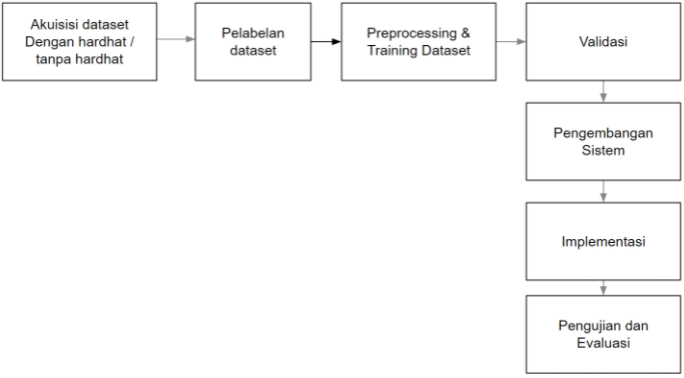
\includegraphics{gambar/blockdiagram-helmetdetection.png}
  \caption{Block Diagram Helmet Detection}
  \label{fig:helmetdetectiondiagram}
\end{figure}

\section{Desain Sistem}
\par Judul ini merupakan penelitian di bidang \emph{computer vision} 


\section{Deskripsi Sistem}
\label{sec:deskripsisistem}

Sistem akan dibuat dengan \lipsum[1-2]

\section{Implementasi Alat
\label{sec:implementasi alat}}

Alat diimplementasikan dengan \lipsum[1]

% Contoh pembuatan potongan kode
\begin{lstlisting}[
  language=C++,
  caption={Program halo dunia.},
  label={lst:halodunia}
]
#include <iostream>

int main() {
    std::cout << "Halo Dunia!";
    return 0;
}
\end{lstlisting}

\lipsum[2-3]

% Contoh input potongan kode dari file
\lstinputlisting[
  language=Python,
  caption={Program perhitungan bilangan prima.},
  label={lst:bilanganprima}
]{program/bilangan-prima.py}

\lipsum[4]
